\documentclass{article}
\usepackage{fullpage}
\usepackage{pgffor}
\usepackage{amssymb}
\usepackage{bm}
\usepackage{mathtools}
\usepackage{verbatim}
\usepackage{appendix}
\usepackage{graphicx}
\usepackage[UKenglish]{isodate} % for: \today
\cleanlookdateon                % for: \today

\def\wl{\par \vspace{\baselineskip}\noindent}
\def\beginmyfig{\begin{figure}[htbp]\begin{center}}
\def\endmyfig{\end{center}\end{figure}}
%\def\prodl{\prod\limits_{i=1}^n}
\def\suml{\sum\limits_{i=1}^n}
\def\ds{\displaystyle}

\begin{document}
% my title:
\begin{center}
  \section*{\textbf{Stat637: Multilevel (Hierarchical) Modeling}
    \footnote{https://github.com/luiarthur/Fall2014/blob/master/Stat637/mp}
  }  
  \subsection*{\textbf{Arthur Lui}}
  \subsection*{\noindent\today}
\end{center}

\section{Introduction}
I will review the paper, ``Multilevel (Hierarchical) Modeling: What It Can and Cannot Do".

\section{Summary of the Paper}

\section{How the Paper Relates to Generalized Linear Models}

\section{Fitting The Model}
\beginmyfig
  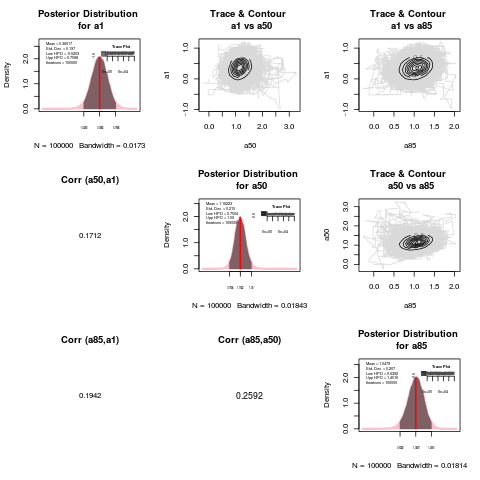
\includegraphics{images/apost.pdf}
\endmyfig

\section{Extending Results of the Paper}

\end{document}
